\tikzstyle{end} = [circle, minimum width = 4pt, fill, inner sep = 1pt,
	opacity = 1]
\tikzstyle{start} = [circle, inner sep = 1pt, opacity = 1]

\onslide<1->{
  	\tikzstyle{startP} = [circle, inner sep = 1pt, opacity = 0]
}
\only<3->{
	\tikzstyle{startP} = [circle, inner sep = 1pt, opacity = 1]
}
            
\tikzstyle{level 1} = [level distance = 0.1cm, sibling distance = 0.4cm]
\tikzstyle{level 2} = [level distance = 0.45cm]
\tikzstyle{level 3} = [level distance = 1cm]
\tikzstyle{level 4} = [level distance = 0.4cm]

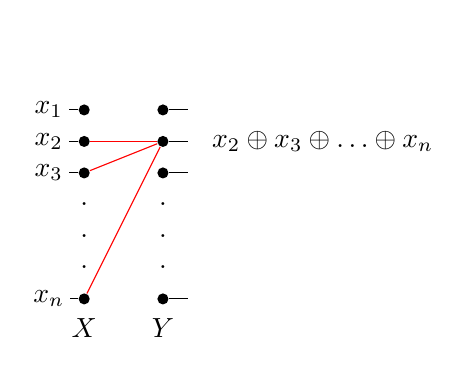
\begin{tikzpicture}[grow = right]
    \node [start]{}
    	child {
        	node [start] (xn) {$x_{n}$}
            	child [end]{
                	node [end] (xvn){}
                    	child [end]{
                        	node [end] (yvn){}
                            	child [start]{
                                	node [start] (yn){}
                                    edge from parent [opacity = 1]
                                }
                            edge from parent [opacity = 0]
                        }
                    edge from parent [opacity = 1]
                }
            edge from parent [opacity = 0]
        }
    	child foreach \i in {3, 2, 1}{
	    	node [start] {}
            	child [start]{
                	node [start] {.}
                    	child [start]{
                        	node [start] {.}
                            edge from parent [opacity = 0]
                        }
                    edge from parent [opacity = 0]
                }
            edge from parent [opacity = 0]
        }
    	child foreach \i in {3, 2, 1}{
	    	node [start] (x\i) {$x_{\i}$}
            	child [end]{
                	node [end] (xv\i){}
                    	child [end]{
                        	node [end] (yv\i){}
                            	child [start]{
                                	node [start] (y\i){}
                                    edge from parent [opacity = 1]
                                }
                            edge from parent [opacity = 0]
                        }
                    edge from parent [opacity = 1]
                }
            edge from parent [opacity = 0]
        };

    \path [draw = red, opacity = 1](xv2) -- (yv2);
    \path [draw = red, opacity = 1](xv3) -- (yv2);
    \path [draw = red, opacity = 1](xvn) -- (yv2);
    \node at (xvn.south) [below = 0.05cm] {$X$};
    \node at (yvn.south) [below = 0.05cm] {$Y$};
    \node at (y2.east) [startP, right = 0.1cm] {$x_{2} \oplus x_{3}
	    \oplus \dots \oplus x_{n}$};
\end{tikzpicture}
